\section{Verifying DaisyNFS using Dafny}
\label{sec:daisy:proof}

A key contribution of DaisyNFS is a proof structure that isolates concurrency and crash
reasoning to the transaction system. The proof works in two steps. First, a
\emph{simulation transfer} theorem extends GoTxn's program refinement to show
how transactions enable sequential reasoning for an arbitrary system implemented
top (\cref{sec:daisy:simulation-transfer}). Second, the sequential reasoning
is implemented and verified in Dafny for the specific case of DaisyNFS and its
NFS specification (\cref{sec:daisy:proof-dafny}).

\subsection{Simulation transfer}%
\label{sec:daisy:simulation-transfer}

The GoTxn specification from \cref{sec:txn:spec} uses program refinement to
capture that transactions are atomic in the sense that every interleaved
execution has a corresponding execution where each transaction runs all at once.
This section describes a \emph{simulation transfer} theorem, proven in Coq, that
uses program refinement to show how GoTxn enables \emph{sequential
reasoning} for a system implemented with transactions on top.

The idea behind the simulation transfer specification is to express that a system
verified using sequential reasoning for each transaction is also correct when
run concurrently through GoTxn --- intuitively, this follows from the atomicity
provided by program refinement.
% , at which point the sequential reasoning
% applies, but we have a more precise and formal proof in Coq.
To make this precise, we define formally what we mean by
``sequential reasoning''. Suppose we have an
implementation of layer $S$ using operations from $T$. Note that all the proofs
about the transaction system are for an arbitrary system with operations in $S$. The implementation $i$
consists of a function $i(op) : \gooselayer{T}$ for each operation $op \in S$. The statement
$\seqrefinement \targ{T, S}(i)$ says that $i$ is a correct sequential
implementation of $S$ using $T$. To specify correctness under crashes, this
definition refers to $\operatorname{crash}(\sigma, \sigma')$, which is a
layer-specific crash transition that models, for example, clearing the
contents of memory.

\begin{definition}
  The implementation $i : S \to \gooselayer{T}$ is a \emph{sequential
    refinement}, written
  $\seqrefinement \targ{T, S}(i)$, if there exists an abstraction relation
  $R : \Sigma_{S} \to \Sigma_{T} \to \textdom{bool}$ such that: \newline
(1) for every operation
  $op \in S$, the following sequential Hoare triple holds:
  \[
    \hoare{R(\sigma)}{i(op)}{\exists \sigma'.\, R(\sigma') \land \sigma \overset{op}{\leadsto} \sigma'},
  \]
(2) $\mathrm{init}(\sigma_{S}, \sigma_{T})$ implies
$R(\sigma_{S}, \sigma_{T})$, and \\
(3) if $R(\sigma_{T}, \sigma_{S})$ holds and $\operatorname{crash}(\sigma_{T}$, $\sigma_{T}')$,
then there exists a $\sigma_{S}'$ such that $R(\sigma_{T}', \sigma_{S}')$ and
$\operatorname{crash}(\sigma_{S}, \sigma_{S}')$.%
  \label{def:seqrefinement}
\end{definition}
%
Conditions (1) and (2) in this definition are standard for sequential
verification of refinement, while condition (3) is a standard condition for sequential crash-safety~\citep{chajed:argosy}. Though condition (3) requires the
abstraction relation to be preserved by crashes, the proof engineer does \emph{not} have to reason about crashes in the middle of operations.
% is a standard condition for sequential crash-safety~\cite{chajed:argosy}
% for sequential crash safety~\cite{chajed:argosy}.
The
diagram in \cref{fig:refinement} depicts the main
refinement condition (1) diagrammatically.
% For example, it is fairly easy to use them to show
% that for any sequential program $p : \gooselayer{S}$, the traces of the code
% $\mathrm{link}(p, i)$ are a subset of the traces of the spec $p$ (we will not
% use exactly this theorem since we are interested in concurrent code using
% transactions).
% \tej{I mentioned this but maybe we don't want/need to say it?}. Such reasoning would be familiar in previous sequential verified
% systems like FSCQ~\cite{chen:fscq}, IronFleet~\cite{hawblitzel:ironfleet}, and
% VeriBetrKV~\cite{hance:veribetrkv}.

The correctness theorem for GoTxn takes a proof of \emph{sequential} refinement
conditions for a system implemented using transactions and derives a \emph{concurrent and crash-safe} refinement.
A transaction must satisfy some conditions to ensure atomicity. We write
$\mathrm{safe}(p)$ to say that $p$ is a valid transaction. The main
restriction is that $p$ cannot access global state such as the heap, since
the transaction system does not make such accesses atomic; further details are
discussed in \cref{sec:txn:program-refinement}.

The theorem uses
$\atomiccomp i$ to represent a substitution that replaces each operation with
its implementation as a transaction; that is,
$(\atomiccomp i)(op) = \atomically{i(op)}$. $\atomically{i(op)}$ represents an
abstract transaction at the Txn layer, which corresponds to a pattern like the
following when linked with the actual GoTxn implementation (this code snippet
uses Go's support for generics, introduced in version 1.18):

\begin{minted}{go}
type txnBody[T] =
  func(tx *Txn) (v T, ok bool)
func runTxn[T](f txnBody[T]) (v T, ok bool) {
  tx := Begin()
  v, ok := f(tx)
  if ok {
    tx.Commit()
  } else {
    tx.Abort()
  }
  return v, ok
}
\end{minted}

\begin{theorem}[Simulation transfer]
  Let $\textdom{Sys}$ be a layer implemented using transactions with
$i : \textdom{Sys} \to \gooselayer{Txn}$, such that
$\seqrefinement\targ{\gooselayer{Txn}, \textdom{Sys}}(i)$ and
$\forall op.\, \mathrm{safe}(i(op))$ hold. Then
\[
  \forall p : \gooselayer{Sys}, \linked{\mathrm{link}(p, \atomiccomp i)} \refines p.
\]
\label{thm:gotxn-transfer}
\end{theorem}

The theorem assumes only an implementation $i$ which gives the body of each
operation in $\mathit{Sys}$ as a transaction. It then gives a refinement in the
style of program refinement for an arbitrary program $p$ that uses the
$\mathit{Sys}$ API, such as the server loop seen in
\cref{sec:daisy:refinement-spec}. The conclusion is a refinement whose
right-hand side is the program $p$ at the top-most abstraction level of the
system. The left-hand side is the executable code for this program, derived in
two steps: first $\mathrm{link}(p, \atomiccomp i)$ takes each abstract operation
$op$ in $p$ and replaces it with $\atomically{i(op)}$, and second
$\linked{\mathrm{link}(p, \atomiccomp i)}$ takes the result of this process and
further replaces $\atomically{i(op)}$ with executable code that uses the GoTxn
implementation for each call to the Txn API and the \cc{runTxn} pattern above to
make the snippet atomic. The overall refinement says that this executable code
has a subset of behaviors of $p$, so that each operation is not only atomic but
follows the abstract specification of the $\mathit{Sys}$ layer.

\subsection{Using simulation transfer with Dafny}%
\label{sec:daisy:proof-dafny}

\newlength{\stepw}
\newlength{\dstepw}
\newlength{\nfstop}

Simulation transfer reduces verifying DaisyNFS's correctness to reasoning about
the transaction that implements each NFS operation. Because this reasoning is
sequential, we carry it out in Dafny, a verification-oriented programming language.
Let $i_{\mathrm{NFS}} : \mathrm{NFS} \to \gooselayer{Txn}$ denote a model of the
Dafny implementation of each NFS operation, as a program using the GoTxn
interface. Note that this is merely a hypothetical model of the Dafny code,
since Goose does not support enough of Go to explicitly construct these terms in
GooseLang. The Dafny annotations on these methods prove sequential refinement
conditions that we will denote $\seqrefinement_{\mathrm{dfy}}(i)$, as
illustrated in \cref{fig:refinement}. This sequential refinement is intended to
encode as precisely as possible the conditions of sequential refinement in the
simulation-transfer theorem, but formally they are distinct since the
definitions are in different formal systems.

\begin{theorem} $\seqrefinement_{\mathrm{dfy}}(i_{\mathrm{NFS}})$ holds, as checked by Dafny.
  \label{thm:dafny}
\end{theorem}

\begin{figure}
  \centering
  \begin{subfigure}{0.25\textwidth}
    \begin{tikzpicture}[>=latex, every node/.append style={}]

  \tikzstyle{exspecstate}=[circle,draw, dashed,minimum size=2mm,fill=gray!20]
  \tikzstyle{specstate}=[circle,draw,minimum size=2mm,fill=gray!20]
  \tikzstyle{nfsstate}=[circle,draw,minimum size=2mm]
  \tikzstyle{sim}=[-]
  \tikzstyle{exsim}=[-, dashed]
  \tikzstyle{stepr}=[thick,->]
  \tikzstyle{exstepr}=[thick,->, dashed]

  \setlength{\stepw}{.75cm}
  \setlength{\dstepw}{\stepw*2}
  \setlength{\nfstop}{0cm}
  \newlength{\spectop}{1cm}
  \setlength{\spectop}{1cm}

  \draw node (N0) at (0,\nfstop) [nfsstate] {};
  \draw node (N1) at (\stepw,\nfstop) [nfsstate] {};
  \draw node (N2) at (\stepw*2,\nfstop) [nfsstate] {};
  \draw node (N3) at (\stepw*3,\nfstop) [nfsstate] {};

  \draw [stepr] (N0.east) -- (N1.west) node[midway] {};
  \draw [stepr] (N1.east) -- (N2.west) node[midway,below=.3] {\code{CREATE}};
  \draw [stepr] (N2.east) -- (N3.west) node[midway] {};

  \draw node (S0) at (0,\spectop) [specstate] {};
  \draw node (S1) at (\stepw*3,\spectop) [exspecstate] {};
  \draw [exstepr] (S0.east) -- (S1.west) node[midway, above=.2] {\code{nfs3create_spec}};

  \draw [sim] (S0.south) -- (N0.north) node[midway,left=.1] {$R$};
  \draw [exsim] (S1.south) -- (N3.north) node[midway,right=.1] {$R$};

\end{tikzpicture}

  %  \caption{Diagram view of sequential refinement.}%
  %  \label{fig:refinement:diagram}%
  \end{subfigure}~~~\vrule~~~~%
\begin{subfigure}{0.3\textwidth}
  {\small
\begin{verbatim}

method CREATE(d_ino: uint64,
              name: Bytes)
 returns (r: Result<Ino>)
 requires R(txn_disk, fs)
 ensures R(txn_disk, fs)
 ensures r.Ok? ==>
 nfs3create_spec(d_ino, name,
   old(fs), fs, r.v)
\end{verbatim}
}
  %\caption{Dafny encoding}%
  %\label{fig:refinement:dafny}
\end{subfigure}
  \caption[Illustration of sequential refinement and its Dafny encoding]%
  {Illustration of $\seqrefinement(i_{NFS})$ (left) and its encoding
in Dafny $\seqrefinement_{\mathrm{dfy}}(i_{NFS})$ (right), for one particular operation.
In the diagram, the solid parts are assumed, and the
dashed parts must be shown to exist. The complete Dafny spec is more precise about
errors.}
  \label{fig:refinement}
\end{figure}

\tej{now can say what Dafny sequential refinement has to say about
initialization and recovery here}

The crash refinement condition (3) is
straightforward; crashes have no effect in both the Txn layer and the NFS layers
because they do not have ephemeral state.

\begin{theorem}
  DaisyNFS atomically implements the NFS protocol, formally stated as the
  refinement $\linkedcode \refines \snfs$. Note that
  $\sdfy = \mathrm{link}(\snfs, i_{\mathrm{NFS}})$.
  \label{thm:daisy-correctness}
\end{theorem}

This theorem re-states the specification developed in
\cref{sec:daisy:refinement-spec}. Its proof is a simple on-paper argument that
connects \cref{thm:gotxn-transfer} (which \emph{assumes} a sequential
refinement) to \cref{thm:dafny} (which \emph{proves} this sequential refinement).
\Cref{fig:refinement-execs} illustrates
the intuition for this theorem in terms of an example execution of $\snfs$: the transaction system proof guarantees an
atomic execution while the sequential refinement guarantees the transactions
themselves are correct.

\begin{figure}
  %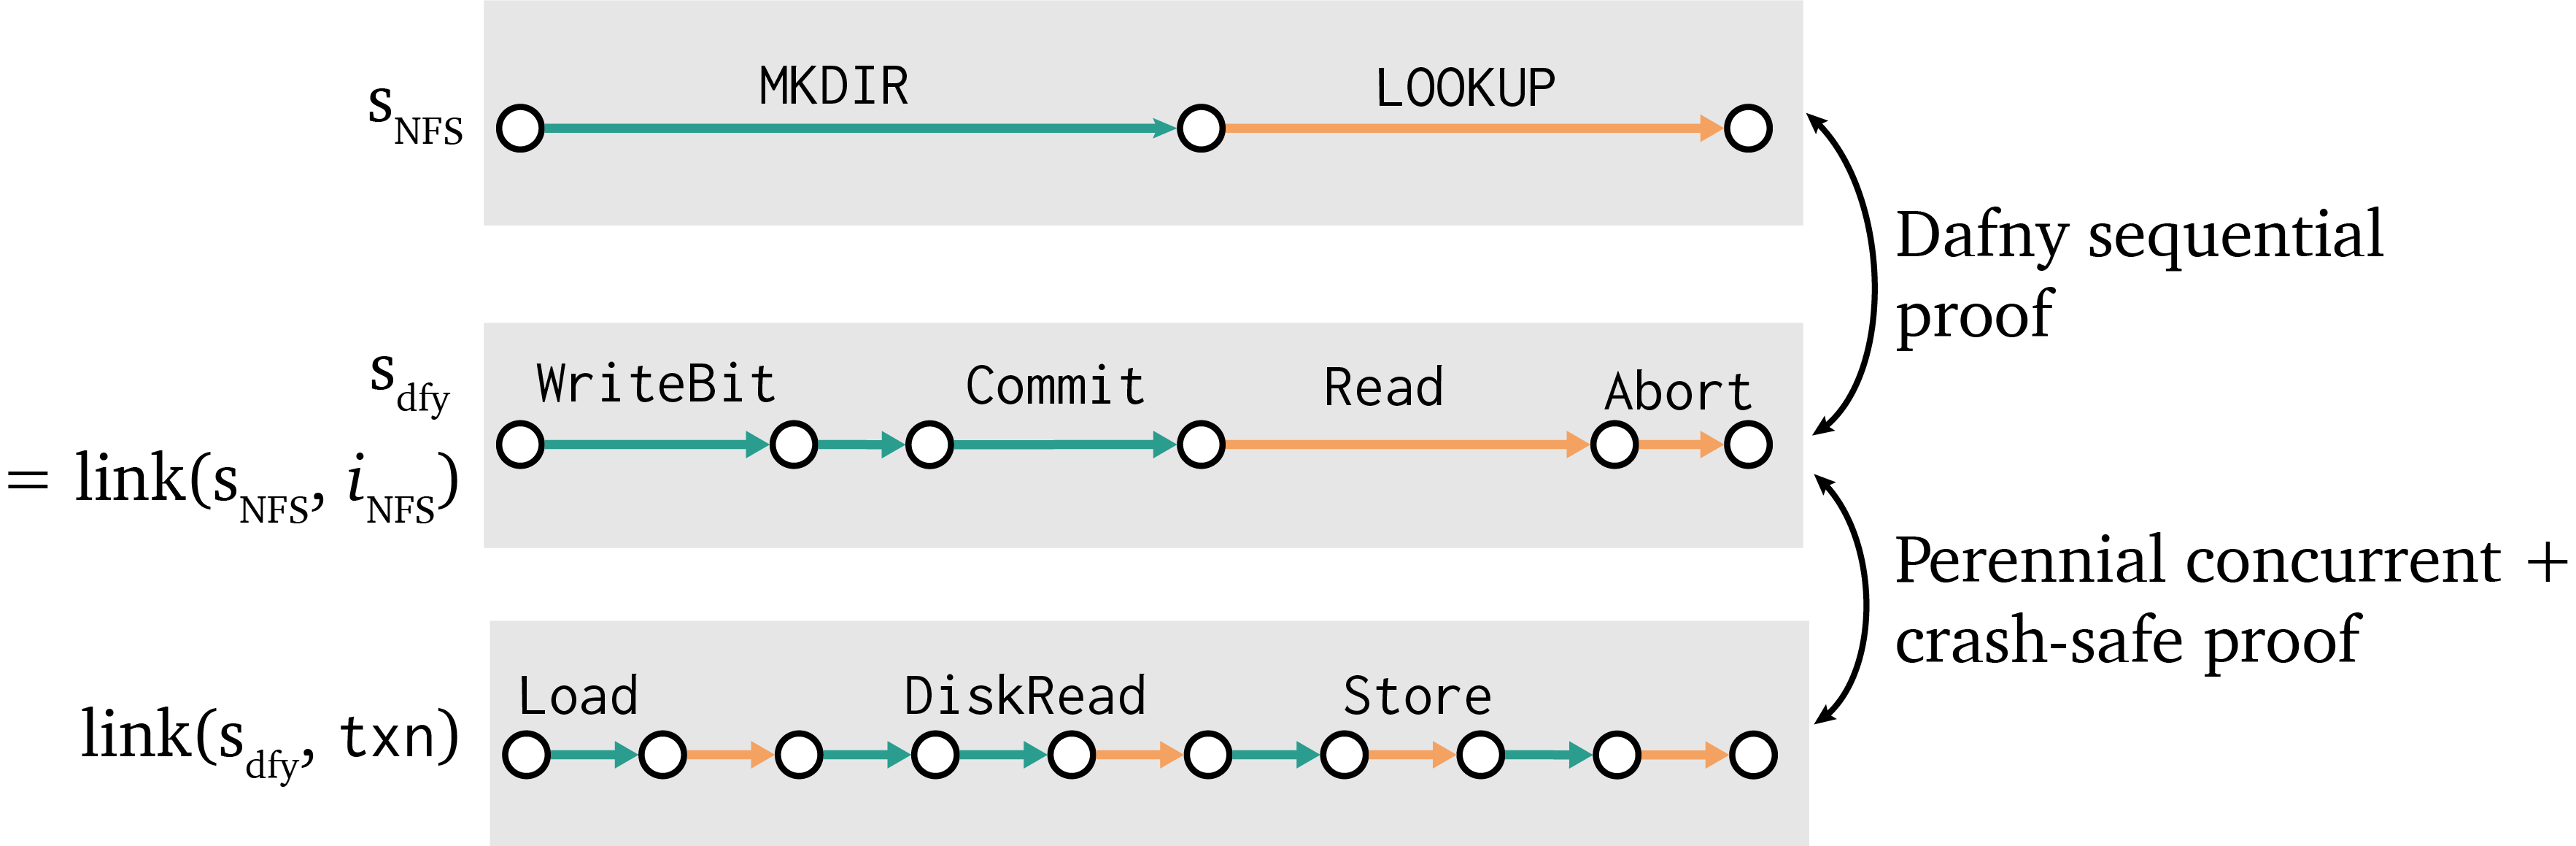
\includegraphics{fig/refinement-execs}
  \begin{center}
  \begin{tikzpicture}[scale=1, >=latex, every node/.append style={}]

  \tikzstyle{txnstate}=[circle,draw,minimum size=2mm,fill=blue!10]
  \tikzstyle{nfsstate}=[circle,draw,minimum size=2mm,fill=yellow!10]
  \tikzstyle{diskstate}=[circle,draw,minimum size=2mm,fill=green!10]
  \tikzstyle{switch}=[->, dashed, dash pattern=on 1.5pt off 2pt]
  \tikzstyle{stepr}=[thick,->]
  \tikzstyle{layer}=[font=\large]

  \setlength{\stepw}{1.25cm}
  \setlength{\dstepw}{\stepw*2}

  \newlength{\nfsbot}
  \newlength{\nfsmid}
  \setlength{\nfstop}{1.5cm}
  \setlength{\nfsbot}{.5cm}
  \setlength{\nfsmid}{(\nfstop+\nfsbot)/2}

  \newlength{\txntop}
  \newlength{\txnbot}
  \newlength{\txnmid}
  \setlength{\txntop}{-.5cm}
  \setlength{\txnbot}{-1.5cm}
  \setlength{\txnmid}{(\txntop+\txnbot)/2}

  \newlength{\disktop}
  \newlength{\diskbot}
  \newlength{\diskmid}
  \setlength{\disktop}{-2.5cm}
  \setlength{\diskbot}{-3.5cm}
  \setlength{\diskmid}{(\disktop+\diskbot)/2}

  \draw node (N0a) at (0,\nfstop) [nfsstate] {};
  \draw node (N1a) at (\dstepw,\nfstop) [nfsstate] {};
  \draw node (N1b) at (\dstepw,\nfsbot) [nfsstate] {};
  \draw node (N2b) at (\dstepw*2,\nfsbot) [nfsstate] {};

  \draw [stepr] (N0a.east) -- (N1a.west) node[midway,above=.2] {\code{LOOKUP}};
  \draw [stepr] (N1b.east) -- (N2b.west) node[midway,above=.2] {\code{CREATE}};
  \draw [switch] (N1a.south) -- (N1b.north);

  \draw node (T0a) at (0,\txntop) [txnstate] {};
  \draw node (T1a) at (\stepw,\txntop) [txnstate] {};
  \draw node (T2a) at (\stepw*2,\txntop) [txnstate] {};
  \draw node (T2b) at (\stepw*2,\txnbot) [txnstate] {};
  \draw node (T3b) at (\stepw*3,\txnbot) [txnstate] {};
  \draw node (T4b) at (\stepw*4,\txnbot) [txnstate] {};

  \draw [stepr] (T0a.east) -- (T1a.west) node[midway,above=.2] {};
  \draw [stepr] (T1a.east) -- (T2a.west) node[midway,above=.2] {\code{Commit}};
  \draw [switch] (T2a.south) -- (T2b.north);
  \draw [stepr] (T2b.east) -- (T3b.west) node[midway,above=.2] {};
  \draw [stepr] (T3b.east) -- (T4b.west) node[midway,above=.2] {\code{Abort}};

  \draw node (D0a) at (0,\disktop) [diskstate] {};
  \draw node (D1a) at (\stepw,\disktop) [diskstate] {};
  \draw node (D1b) at (\stepw,\diskbot) [diskstate] {};
  \draw node (D2b) at (\stepw*2,\diskbot) [diskstate] {};
  \draw node (D3b) at (\stepw*3,\diskbot) [diskstate] {};
  \draw node (D3a) at (\stepw*3,\disktop) [diskstate] {};
  \draw node (D4a) at (\stepw*4,\disktop) [diskstate] {};

  \draw [stepr] (D0a.east) -- (D1a.west) node[midway,above=.2] {\code{Read}};
  \draw [switch] (D1a.south) -- (D1b.north);
  \draw [stepr] (D1b.east) -- (D2b.west) node[midway,above=.2] {\code{Write}};
  \draw [stepr] (D2b.east) -- (D3b.west) node[midway,above=.2] {};
  \draw [switch] (D3b.north) -- (D3a.south);
  \draw [stepr] (D3a.east) -- (D4a.west) node[midway,above=.2] {};

  \draw [align=center] node (NFS) at (\stepw*5.5,\nfsmid) [layer] {$\snfs$ \\ \gooselayer{NFS}};
  \draw [align=center] node (Txn) at (\stepw*5.5,\txnmid) [layer] {$\sdfy$ \\ \gooselayer{Txn}};
  \draw [align=center] node (Disk) at (\stepw*5.5, \diskmid) [layer] {$\linkedcode$ \\ \gooselayer{Disk}};

\end{tikzpicture}

  \end{center}
  \caption[One execution of DaisyNFS at its three abstraction levels]{One possible execution of DaisyNFS, receiving parallel LOOKUP and
    CREATE operations, at its three abstraction levels.
    Within an execution each row is a thread, and dashed arrows indicate
    context switches.
    The proof shows the bottom execution is equivalent to an atomic execution of
    each thread at
    the Txn layer~(in \cref{thm:gotxn-transfer}),
    and sequential reasoning shows each atomic sequence behaves according to the NFS
    specification~(in \cref{thm:dafny}).}
  \label{fig:refinement-execs}
\end{figure}

There are two assumptions needed for the theorems to compose. First,
$\seqrefinement_{\mathrm{dfy}}(i_{NFS})$ should imply $\seqrefinement(i_{NFS})$,
to bridge the assumption and theorem being proven in Dafny. That is, the
encoding of the refinement conditions in Dafny must be correct, but also the
semantics of the transaction system operations modeled in Dafny must match the
Coq proof. Second, every Dafny transaction must be valid, meaning
$\mathrm{safe}(i_{NFS}(op))$. Safety has a static restriction that transactions
should not modify global state, which the Dafny code satisfies because the only
mutable state in the file-system Dafny class is the transaction system, so
file-system operations cannot make mutations other than through GoTxn. The
dynamic restrictions for safety are expressed with preconditions on the GoTxn
interface so that Dafny automatically enforces them.

\tej{subtlety about internal mutable state}

% We have some
% confidence this holds due to a simple check over the Dafny code: the only
% mutable state in the Dafny class that implements the file system is the ghost
% variables and the transaction system, so it cannot make mutations other than
% through GoTxn (ghost variables cannot influence execution due to the design of
% Dafny).
